\section{Funktionen}
	\subsection{Impulsfunktion - Dirac Delta Funktion}
		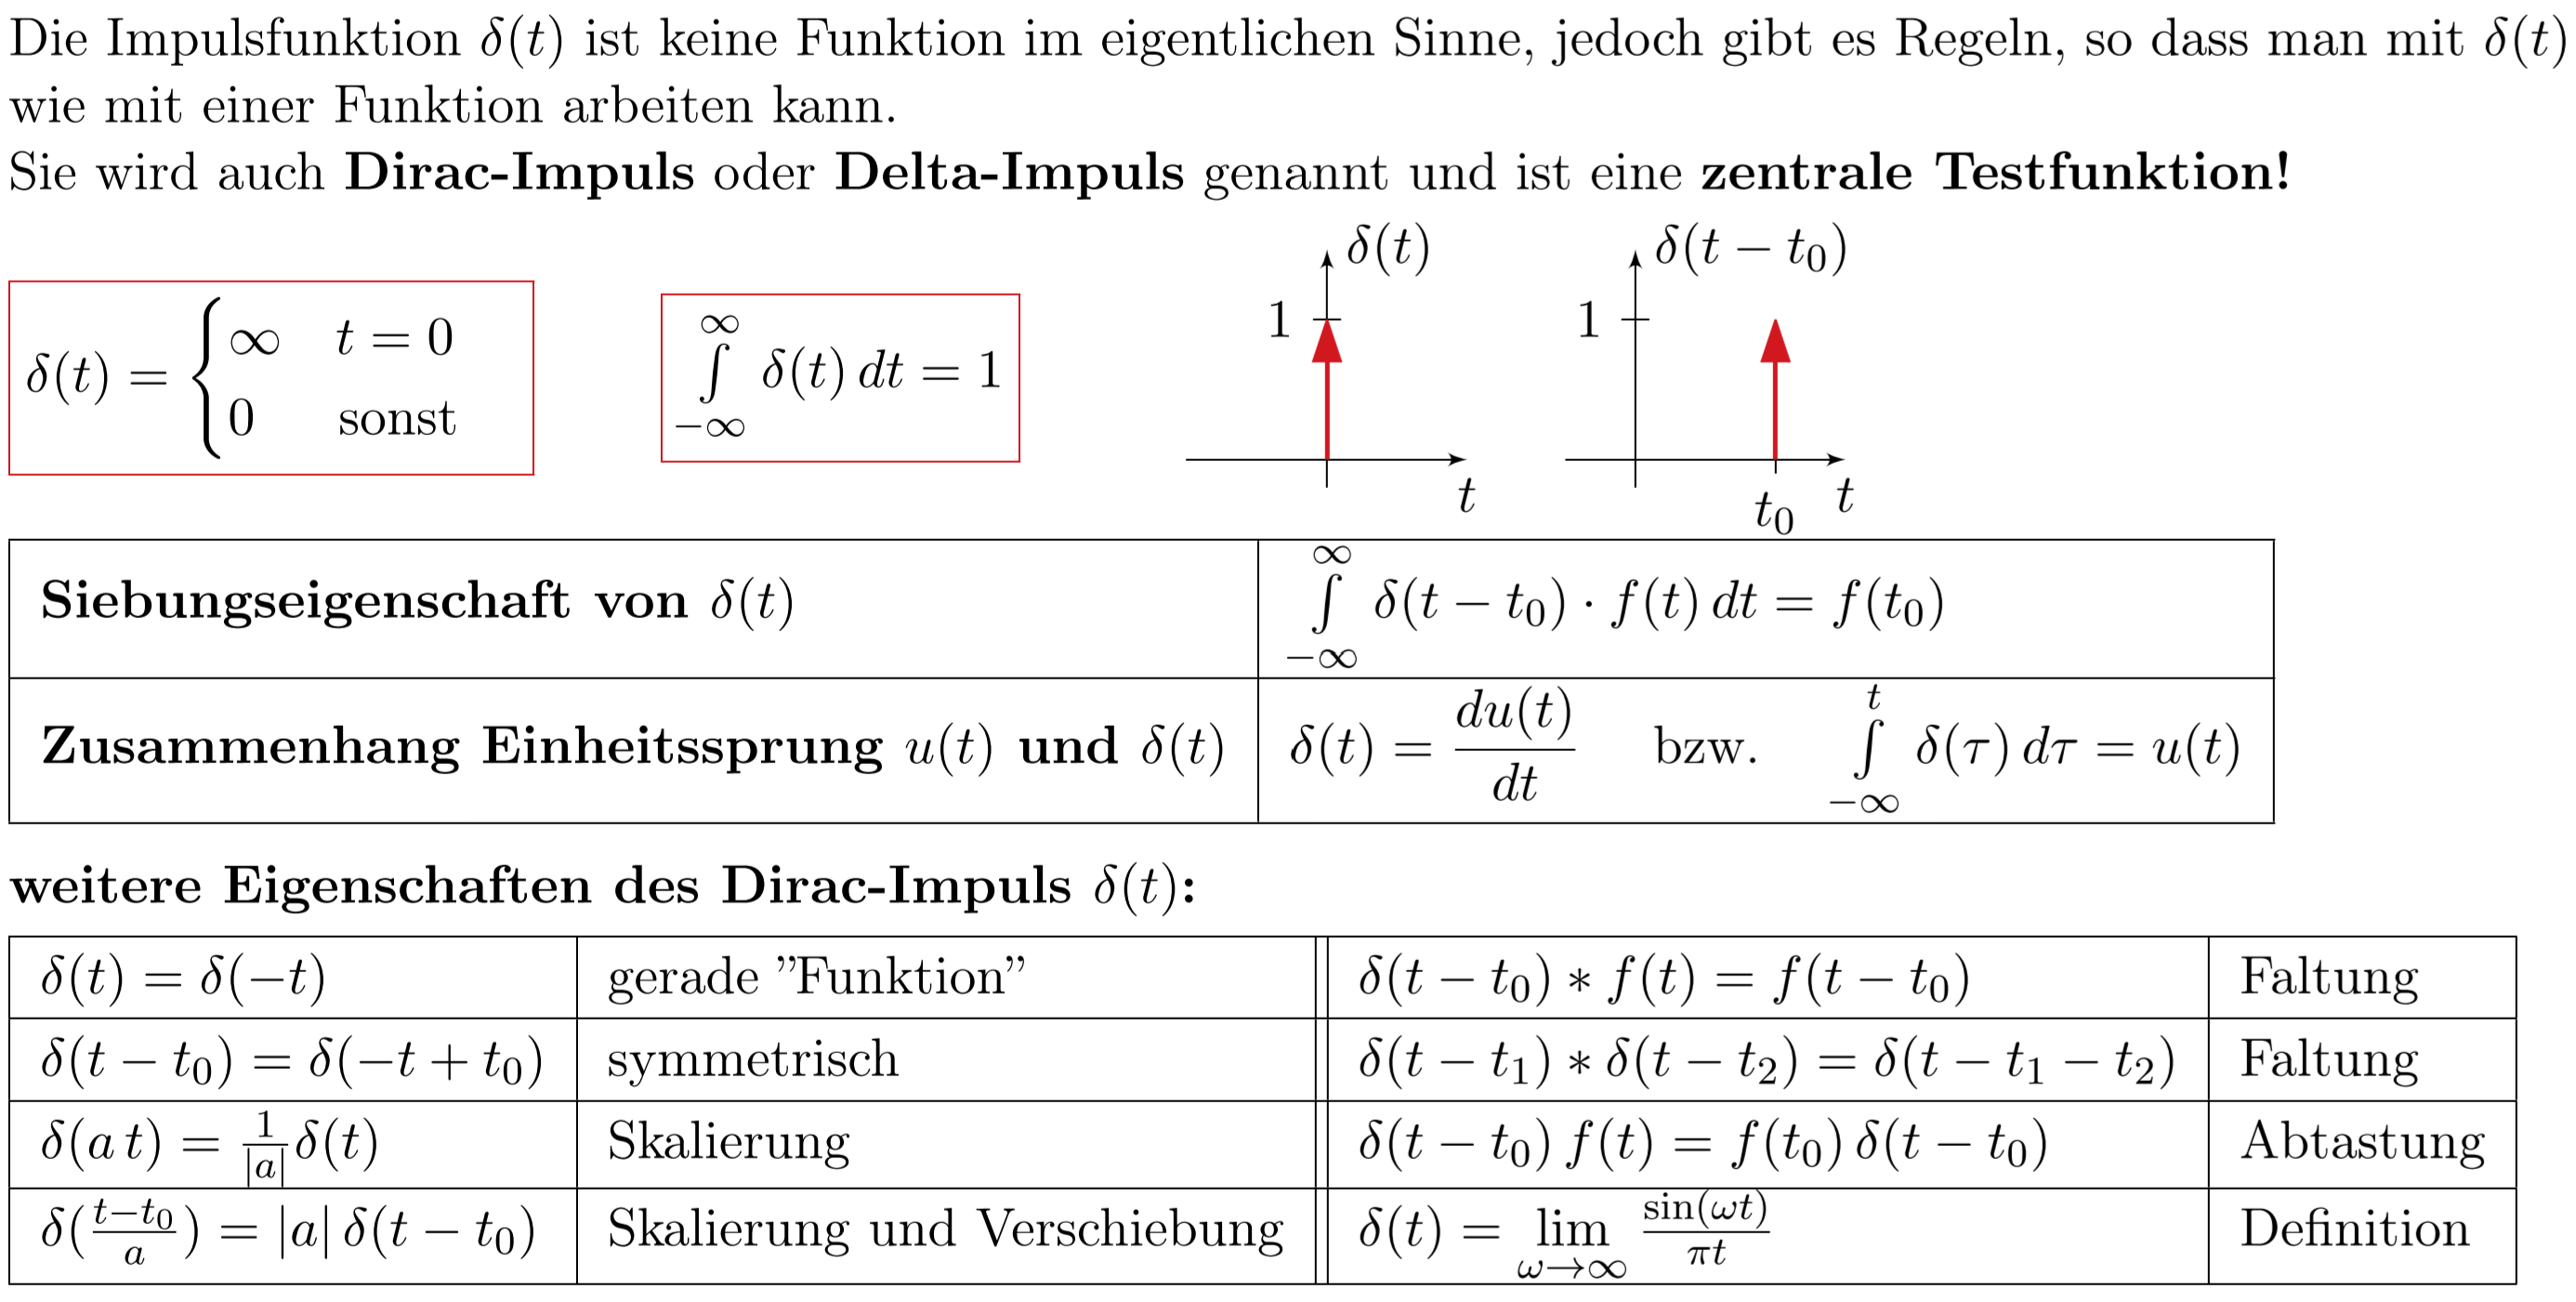
\includegraphics[width=0.8\textwidth]{./bilder/funktionen/impulsF.png}
	
	\subsubsection{Fouriertransformierte $\delta(t)$}
		$\delta(t) \; \laplace \; 1(\omega)$ \qquad
		$\delta(t-t_0) \; \laplace \; e^{-j\omega t_0}$ \qquad
		$1(t) \; \laplace \; 2\pi \delta(\omega)$



	\subsection{Schrittfunktion - unit step}
		\begin{minipage}{0.2\textwidth}
			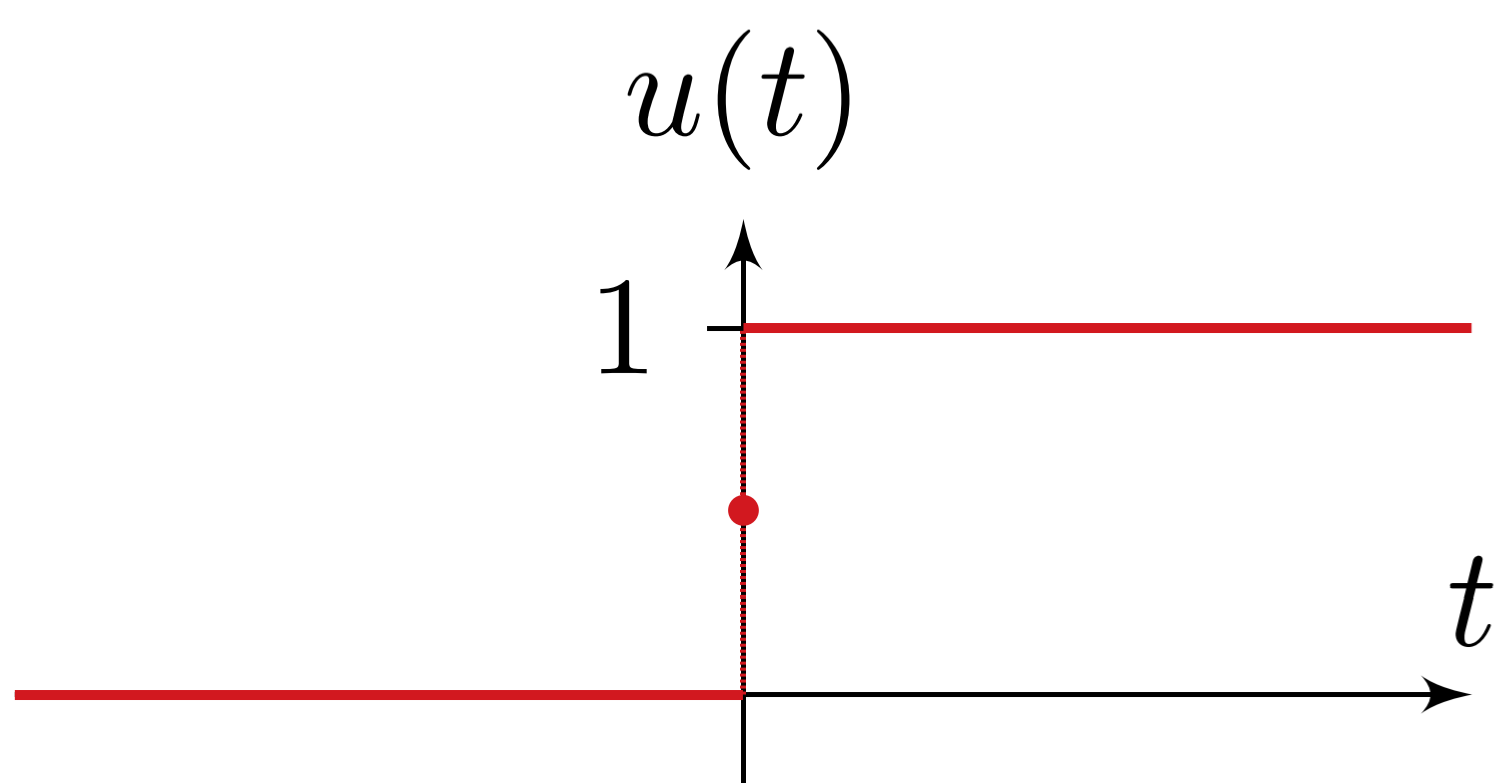
\includegraphics[width=\textwidth]{./bilder/funktionen/sprungF.png}
		\end{minipage}
		\qquad
		\begin{minipage}{0.45\textwidth}
			$u(t) = \sigma(t) =	\begin{cases}
			0 & \text{f\"ur } t < 0 \\
			\frac{1}{2} \text{(praxis)}  \text{ oder undef. (math.)} & \text{f\"ur } t = 0 \\
			1 & \text{f\"ur } t > 0
			\end{cases}$
		\end{minipage}
		\qquad
		\begin{minipage}{0.25\textwidth}						
			$\sigma(t) \; \laplace \; \frac{1}{j\omega} + \pi\delta(\omega) = \Sigma(\omega)$ \\
			\\
			$\frac{du(t)}{dt}=\delta(t)$\\
		\end{minipage}
	
	
	\subsection{Signumfunktion}
		\begin{minipage}{0.2\textwidth}
			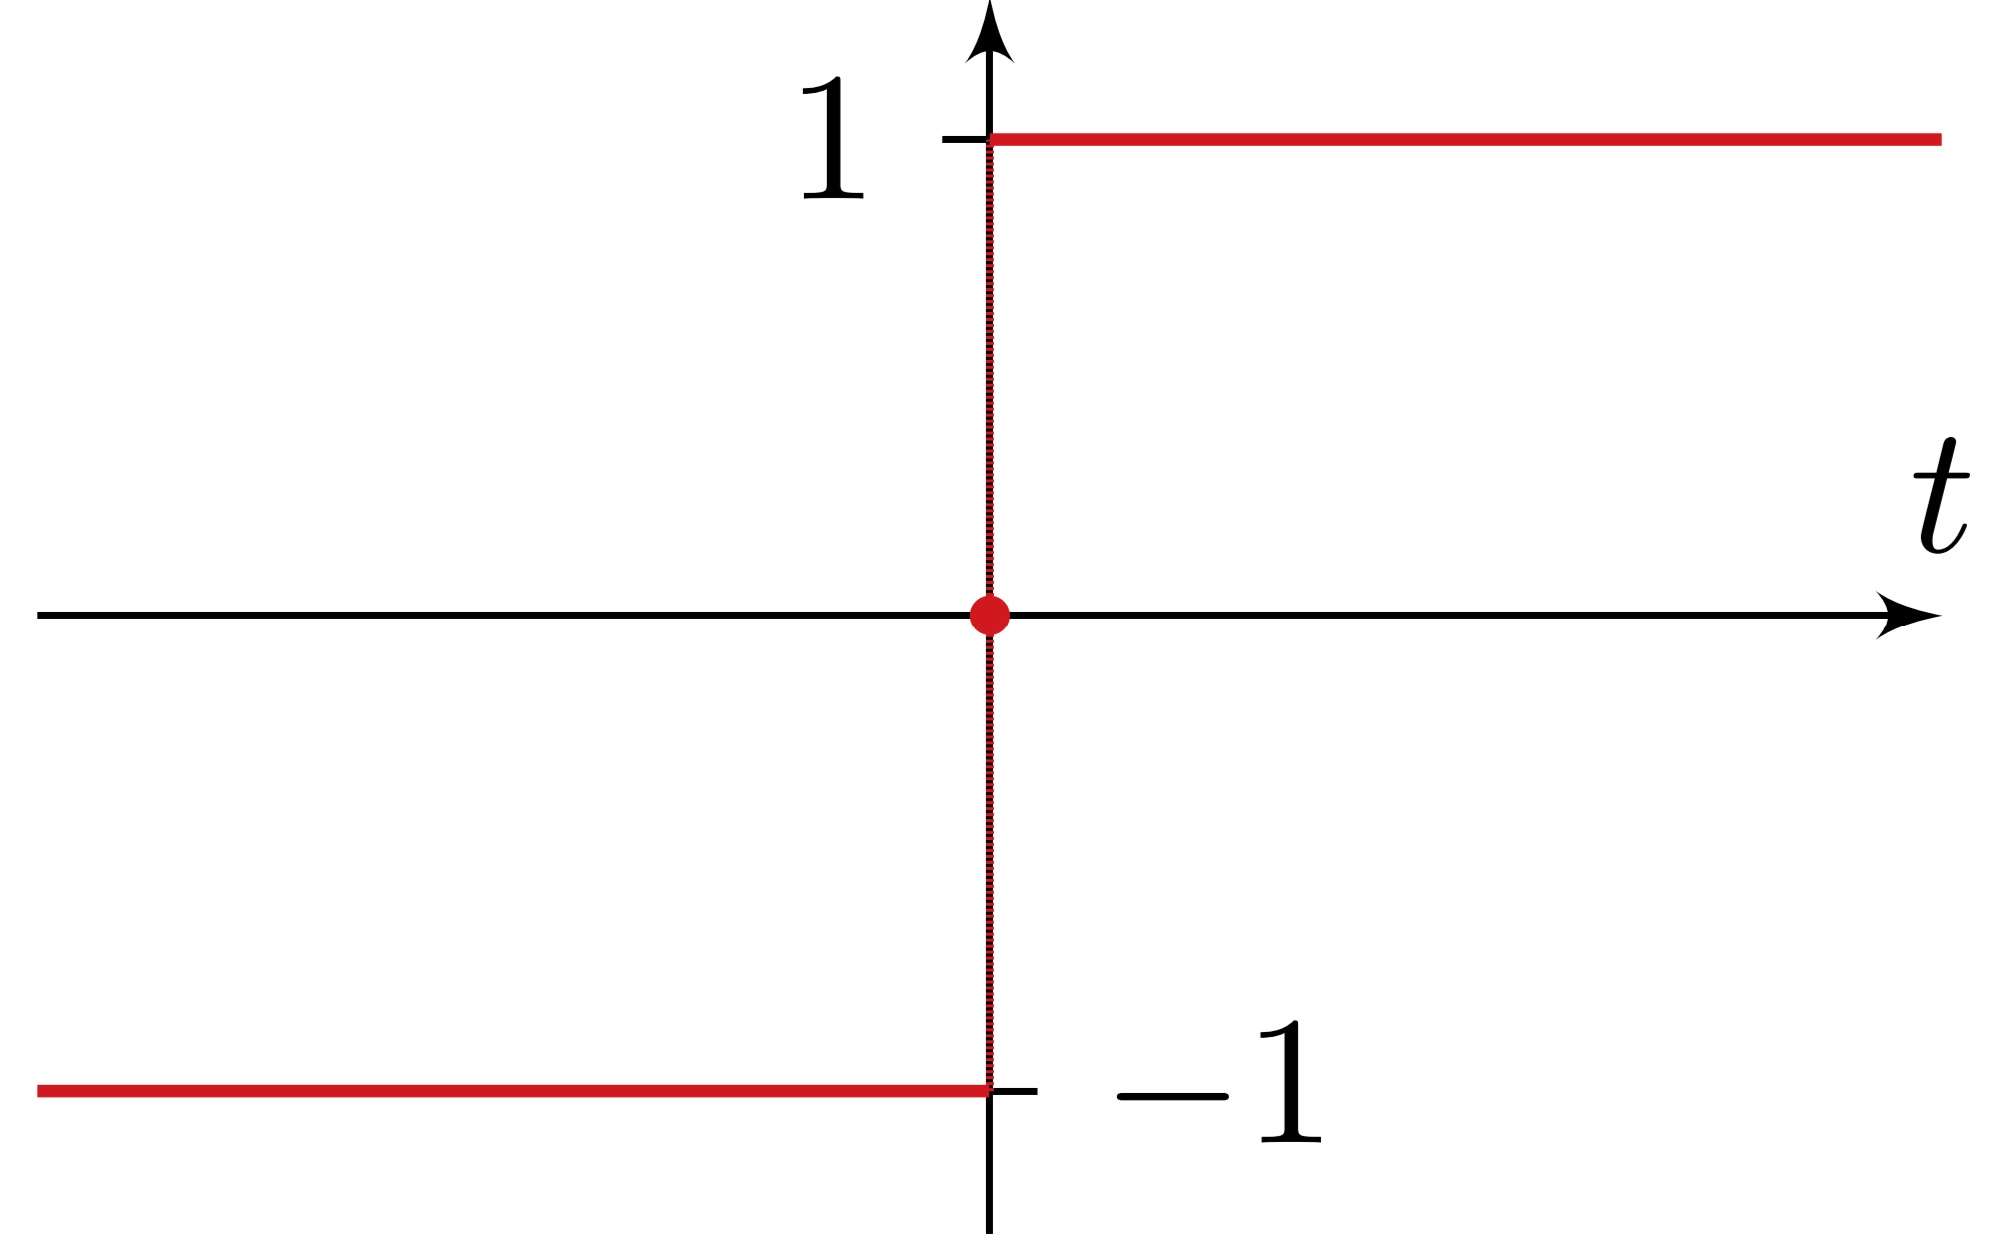
\includegraphics[width=\textwidth]{./bilder/funktionen/signF.png}
		\end{minipage}
		\qquad
		\begin{minipage}{0.45\textwidth}
			$sgn(t) = \begin{cases} 1 & \text{falls }t > 0 \\ -1 & \text{falls }t < 0 \end{cases}$
		\end{minipage}
		\qquad
		\begin{minipage}{0.25\textwidth}						
			$sgn(t) \; \laplace \; \frac{2}{j\omega}$\\
			\\
			$\frac{1}{\pi t} \; \laplace \; -j \cdot sgn(\omega)$\\
		\end{minipage}		

		
	\subsection{Rechteckimpuls}
		\begin{minipage}{0.2\textwidth}
			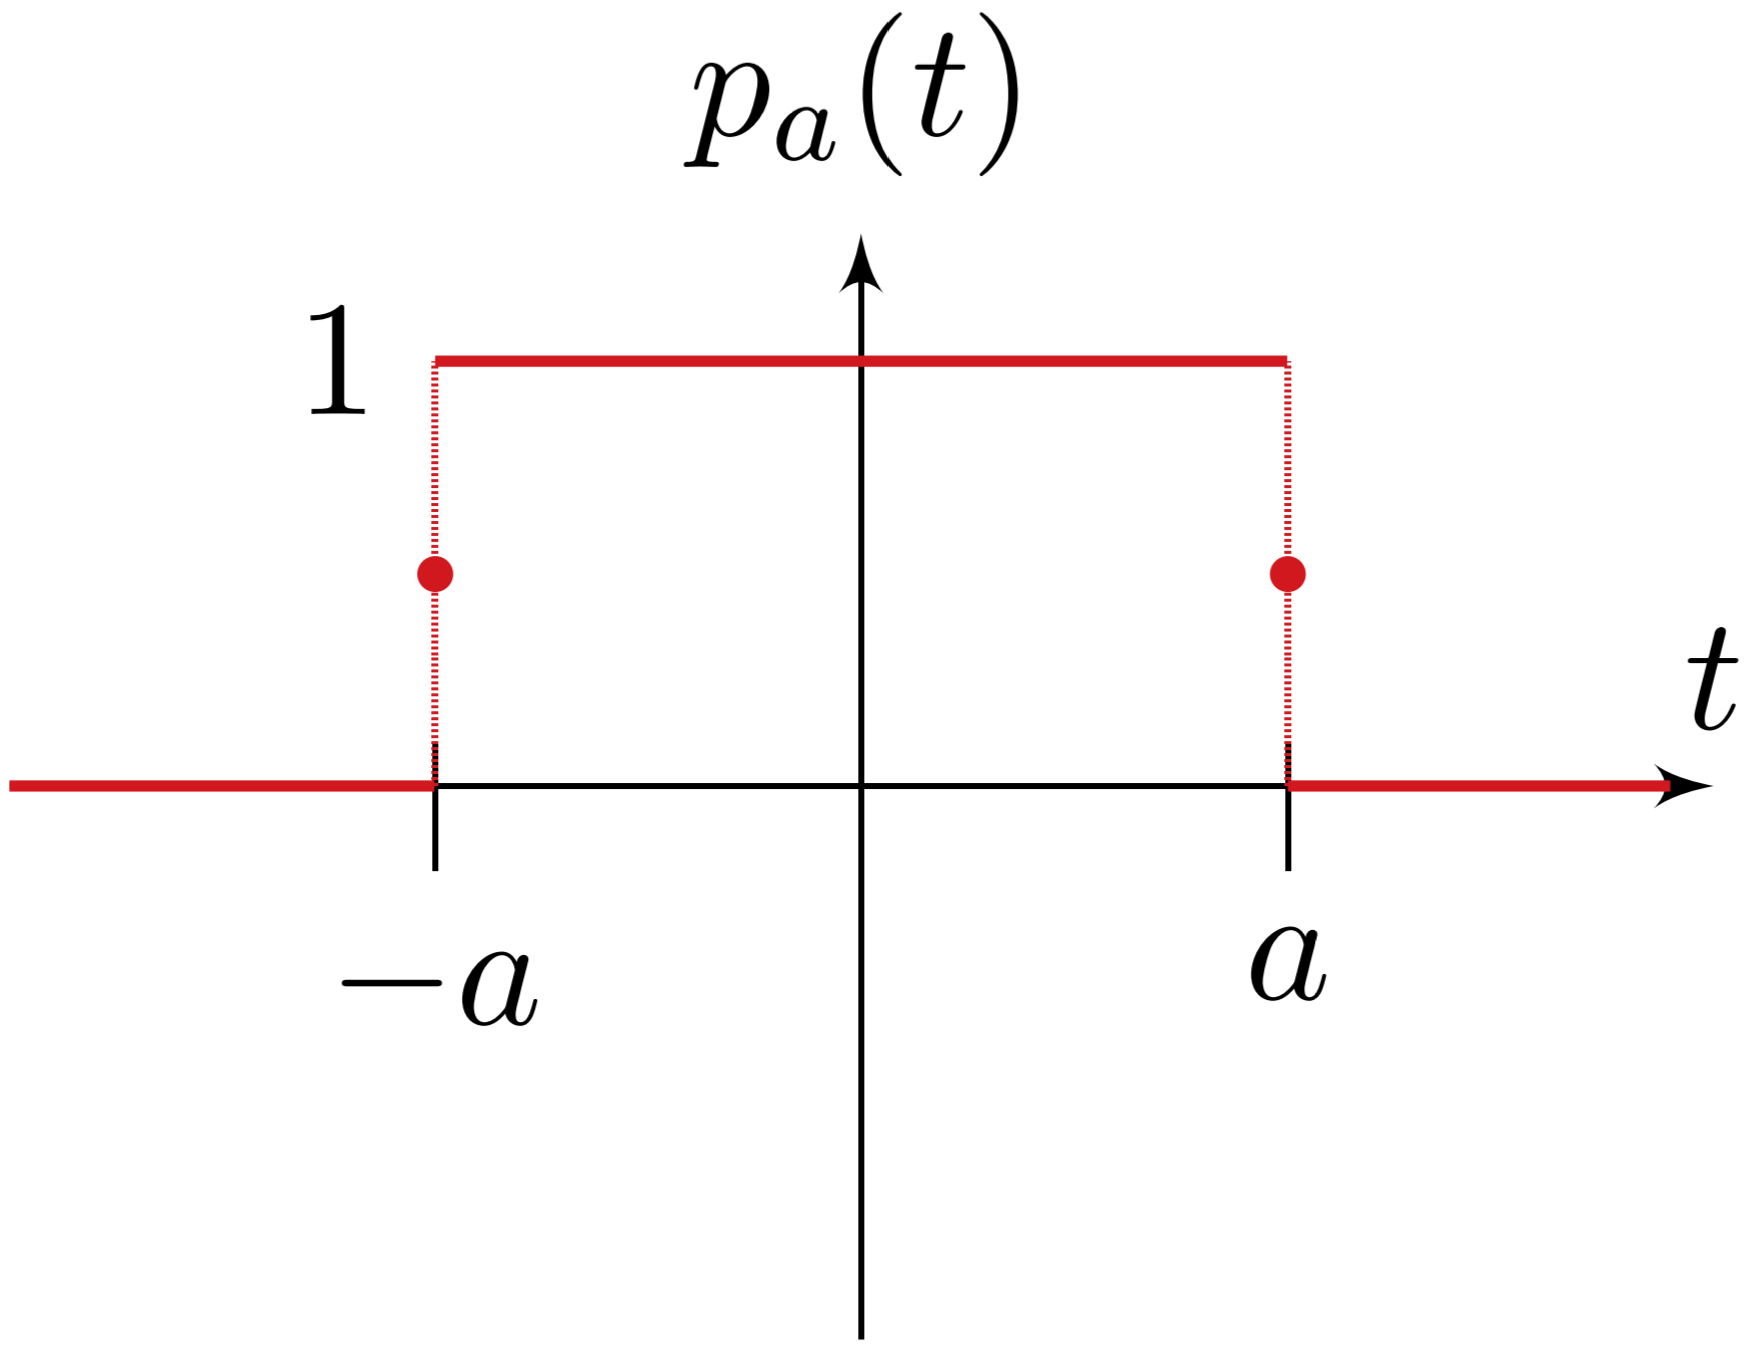
\includegraphics[width=\textwidth]{./bilder/funktionen/rechteckF.png}
		\end{minipage}
		\qquad
		\begin{minipage}{0.45\textwidth}
			$p_{a}(t)=\begin{cases}
							1 & |t|<a \\ 
							\frac{1}{2} & |t|=a \\ 
							0 & |t|>a
						\end{cases}$
		\end{minipage}
		\qquad
		\begin{minipage}{0.25\textwidth}						
			%
		\end{minipage}
	
	\subsection{Rampenfunktion}
		\begin{minipage}{0.2\textwidth}
			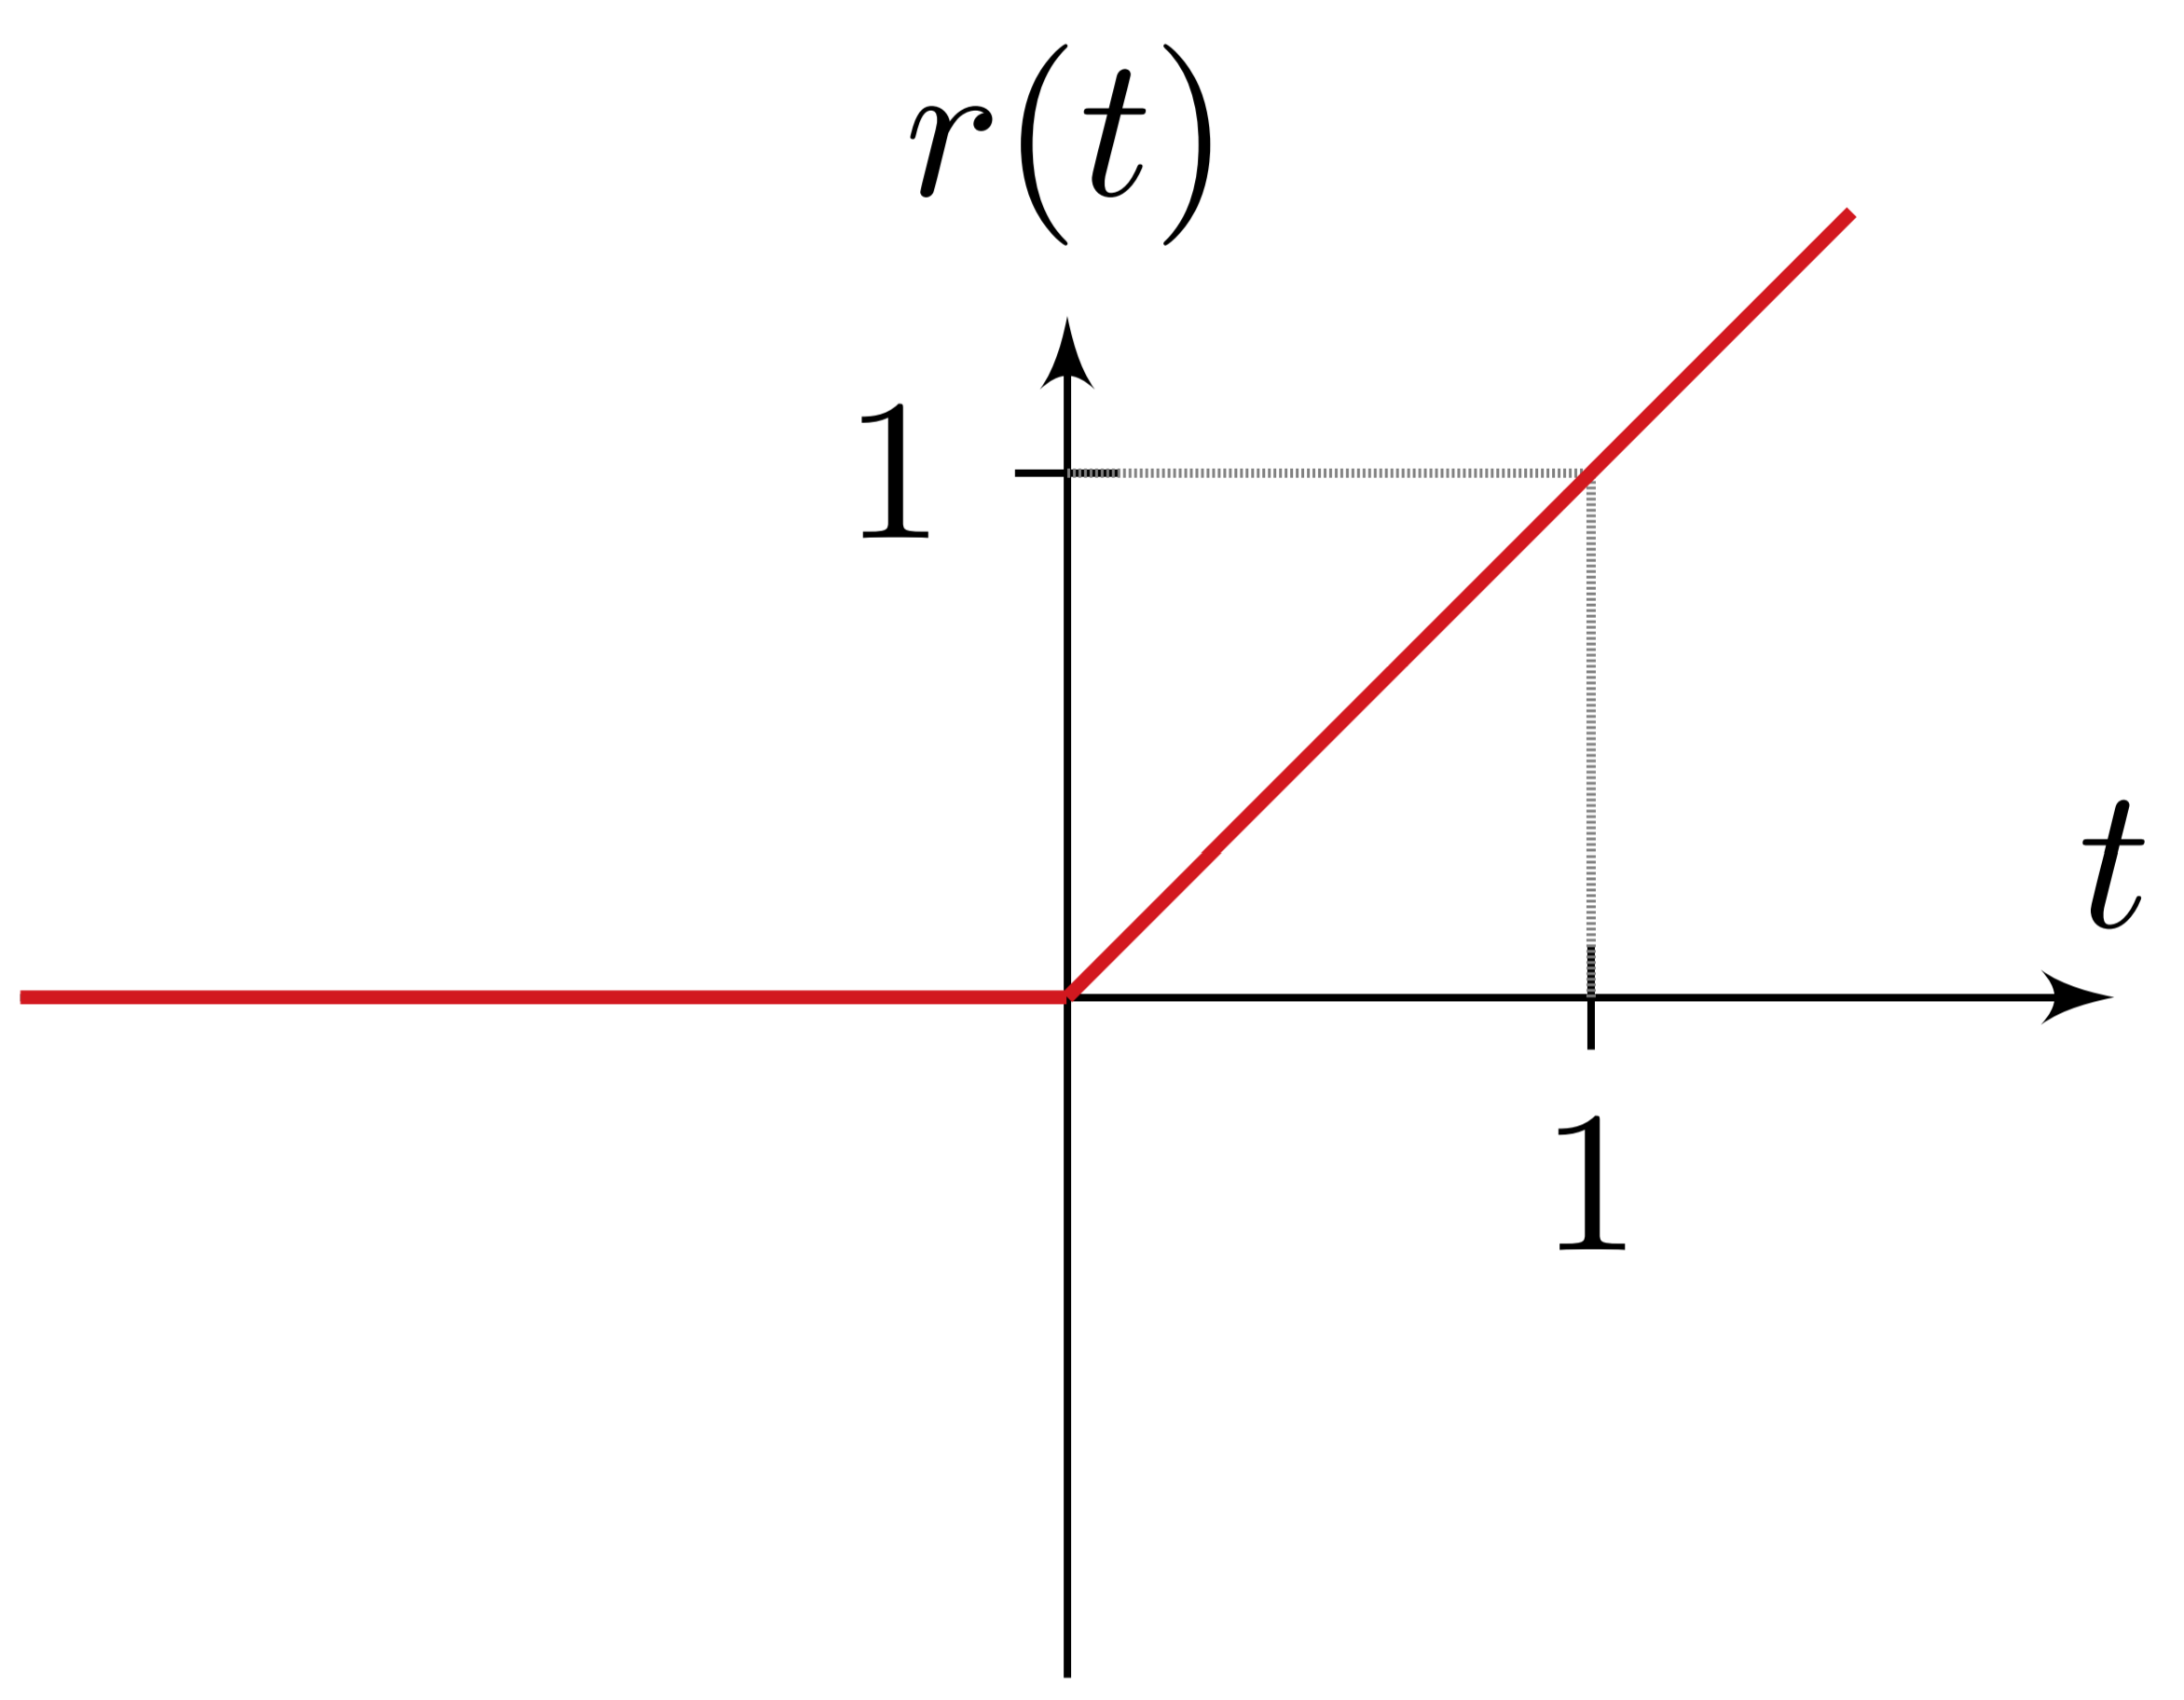
\includegraphics[width=\textwidth]{./bilder/funktionen/rampenF.png}
		\end{minipage}
		\qquad
		\begin{minipage}{0.45\textwidth}
			$r(t)=\begin{cases}
						{0} & {t \leq 0} \\ 
						{t} & {t>0}
					\end{cases}$
		\end{minipage}
		\qquad
		\begin{minipage}{0.25\textwidth}						
			%
		\end{minipage}		
		
	\subsection{Dreieckimpuls}
		\begin{minipage}{0.2\textwidth}
			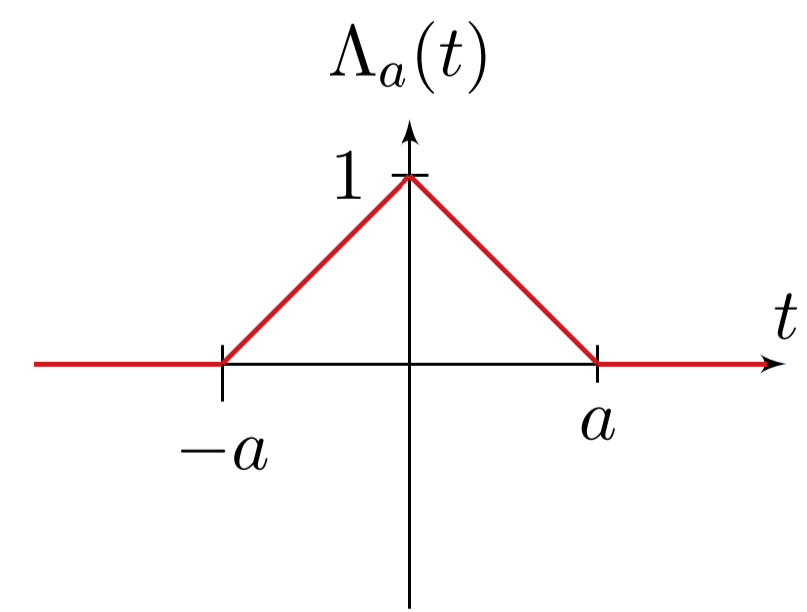
\includegraphics[width=\textwidth]{./bilder/funktionen/dreieckF.png}
		\end{minipage}
		\qquad
		\begin{minipage}{0.45\textwidth}
			$\Lambda_{a}(t)=\begin{cases}{1-\frac{|t|}{a}} & {t<a} \\ {0} & {|t| \geq a}\end{cases}$
		\end{minipage}
		\qquad
		\begin{minipage}{0.25\textwidth}						
			%
		\end{minipage}
	
	
	\subsection{Sinc-Funktion}
				\begin{minipage}{0.2\textwidth}
			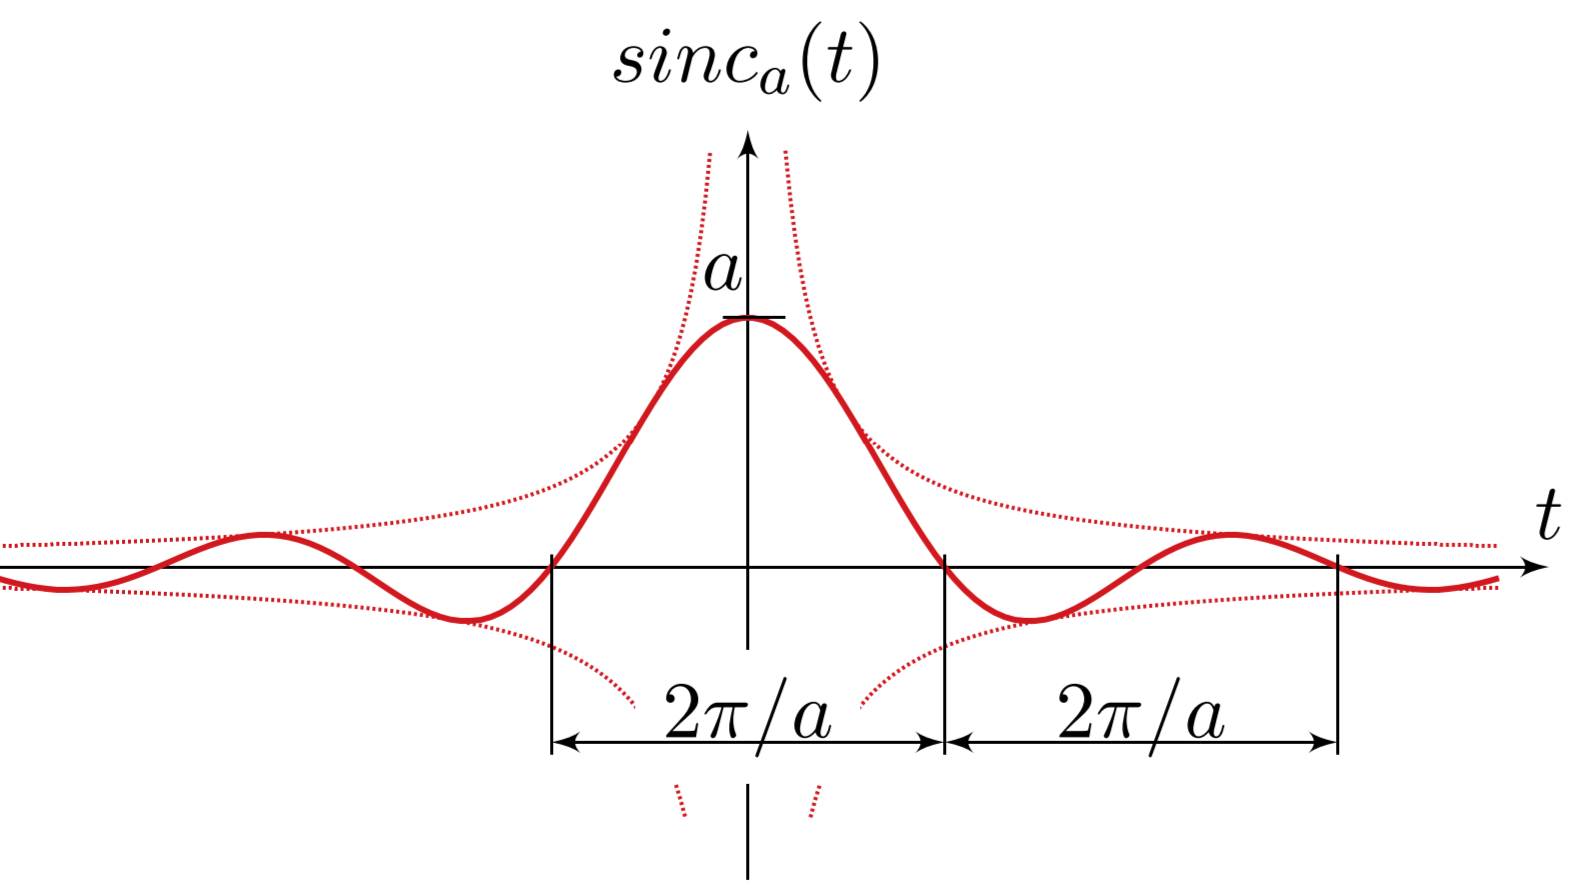
\includegraphics[width=\textwidth]{./bilder/funktionen/sincF.png}
		\end{minipage}
		\qquad
		\begin{minipage}{0.45\textwidth}
			\begin{math}
				\begin{aligned}
					\operatorname{sinc}_{a}(t) &= \frac{\sin (a t)}{t} \\
					\operatorname{sinc}(a t) &= \frac{\sin (a t)}{a t}
				 \end{aligned}
			 \end{math}
		\end{minipage}
		\qquad
		\begin{minipage}{0.25\textwidth}						
			%
		\end{minipage}\\
	
		
		%TODO Berechnungen zu den Funktionen hinzufügen
%		\subsection{Beispiele}
%			\begin{tabular}{l l l}
%				Rechteckimpuls $r_T$ der Breite $2T$ & $r_T \; \laplace \; \frac{2 \cdot \sin(\omega T}{\omega}$ \\
%			\end{tabular}\\
%			\begin{tabular}{p{9cm} p{9cm}}
%				$r_T(t) \; \laplace \; \frac{2}{\omega} \cdot \sin(\omega T) \Rightarrow$ sinc-Funktion &
%				$\int\limits_{-\infty}^{\infty} \frac{\sin(a \omega)}{\omega} d\omega = 
%				\begin{cases} \pi & \text{falls }a > 0 \\ -\pi & \text{falls }a < 0 \end{cases}$
%			\end{tabular}
	
	
	\subsection{Funktionen manipulieren}
		\includegraphics[width=0.8\textwidth]{./bilder/funktionen/SignalManip.png}